\documentclass[titlepage]{article}
\usepackage{adjustbox}
\usepackage{graphicx}
\graphicspath{ {./images/} }


%% DOCUMENT OUTLINE
% Cover Page
% Overview
% What sets the project apart?
% Story and gameplay
% Schedule

%% NOTES FOR CONCEPTUALIZATION 2
% Players	
% 		Singleplayer at first, maybe a second if time allows
% 		If we have a second player:
% 		- Enable two-player puzzles for dungeon generation
% 		- Increase enemy health (maybe x2, but experiment)
% 
% Objective
% 		Find special item and defeat boss in each dungeon
% 
% Procedures
% 		- Player navigates dungeon in 2D space
% 		- Player recovers health by defeating enemies
% 		- Player recovers health by interrupting charge attacks
% 		- Player deals extra damgage by interrupting charge attacks
% 		- Enemies are stunned after charge attacks are interrupted
% 		- The player traverses the world in a 2D side scroller
% 		- Dungeons are randomly generated from preset room templates
% 
% 		- The grappling hook:
% 			- Starts able to pull small enemies
% 			- Can be upgraded to pull larger enemies in skill tree
% 			- Pulls the player towards enemies too large to pull
% 			- Pulls the player towards bosses (always)
% 			- Pulls the player to hook targets
% 
% 		- The staff of blasting:
% 			- explodes on hitting enemies and breakable walls
% 			- upgrade explosion radius and damage in skill tree
% 			- explodes when it runs out of bounces
% 			- deals partial damage to the player if caught in explosion
% 			- starts with two bounces upgraded through skill tree
% 				- Call the upgrade perk "Chaos Theory"
% 			- fires a sphere with a conical tail that shows the path
% 
% Rules	
% 		- One special item room per dungeon
% 		- One boss room per dungeon
% 		- Minion enemies spawn in dungeons and the overwold
% 		- Special items spawn once per world
% 		- Bosses spawn once per world
% 
% Resources
% 		- Health
% 		- Special items charge
% 			- Time to compress grappling hook spring
% 				- Hook has lower range if not full energy
% 			- Time to charge arcane energy in staff of blasting
% 				- Blast is slower and less damage if not full energy
% 		- Experience points (spent on skill tree upgrades)
% 		- Health pickups dropped by minions (must be picked up)
% 
% Conflict
% 		Player vs Game
% 		- Defeating enemies
% 		- Solving puzzles
% 		- Solving navigation
% 
% Boundaries
% 		- Player moves between rooms
% 		- Minions, puzzles, and bosses limited to a single room in dungeons
% 		- Minions in the overwold limited to patrol areas
% 
% Outcome	
% 		Player defeats all the bosses, or they give up.


\title{Shattered Reformation (Working)\\Super Fantasy 7}
\author{Savanna Middaugh, Hannah Murphy, Orion Nassaux, Jacob Santillanes}

\begin{document}
\begin{titlepage}
    \centering
    \vfill
    {\bfseries\Large
        "Shattered Reformation" Design Document\\
        Game by Super Fantasy 7\\
        \vskip2cm
        Savanna Middaugh, Hannah Murphy, Orion Nassaux, Jacob Santillanes\\
	v1.0.0
    }    
    \vfill
    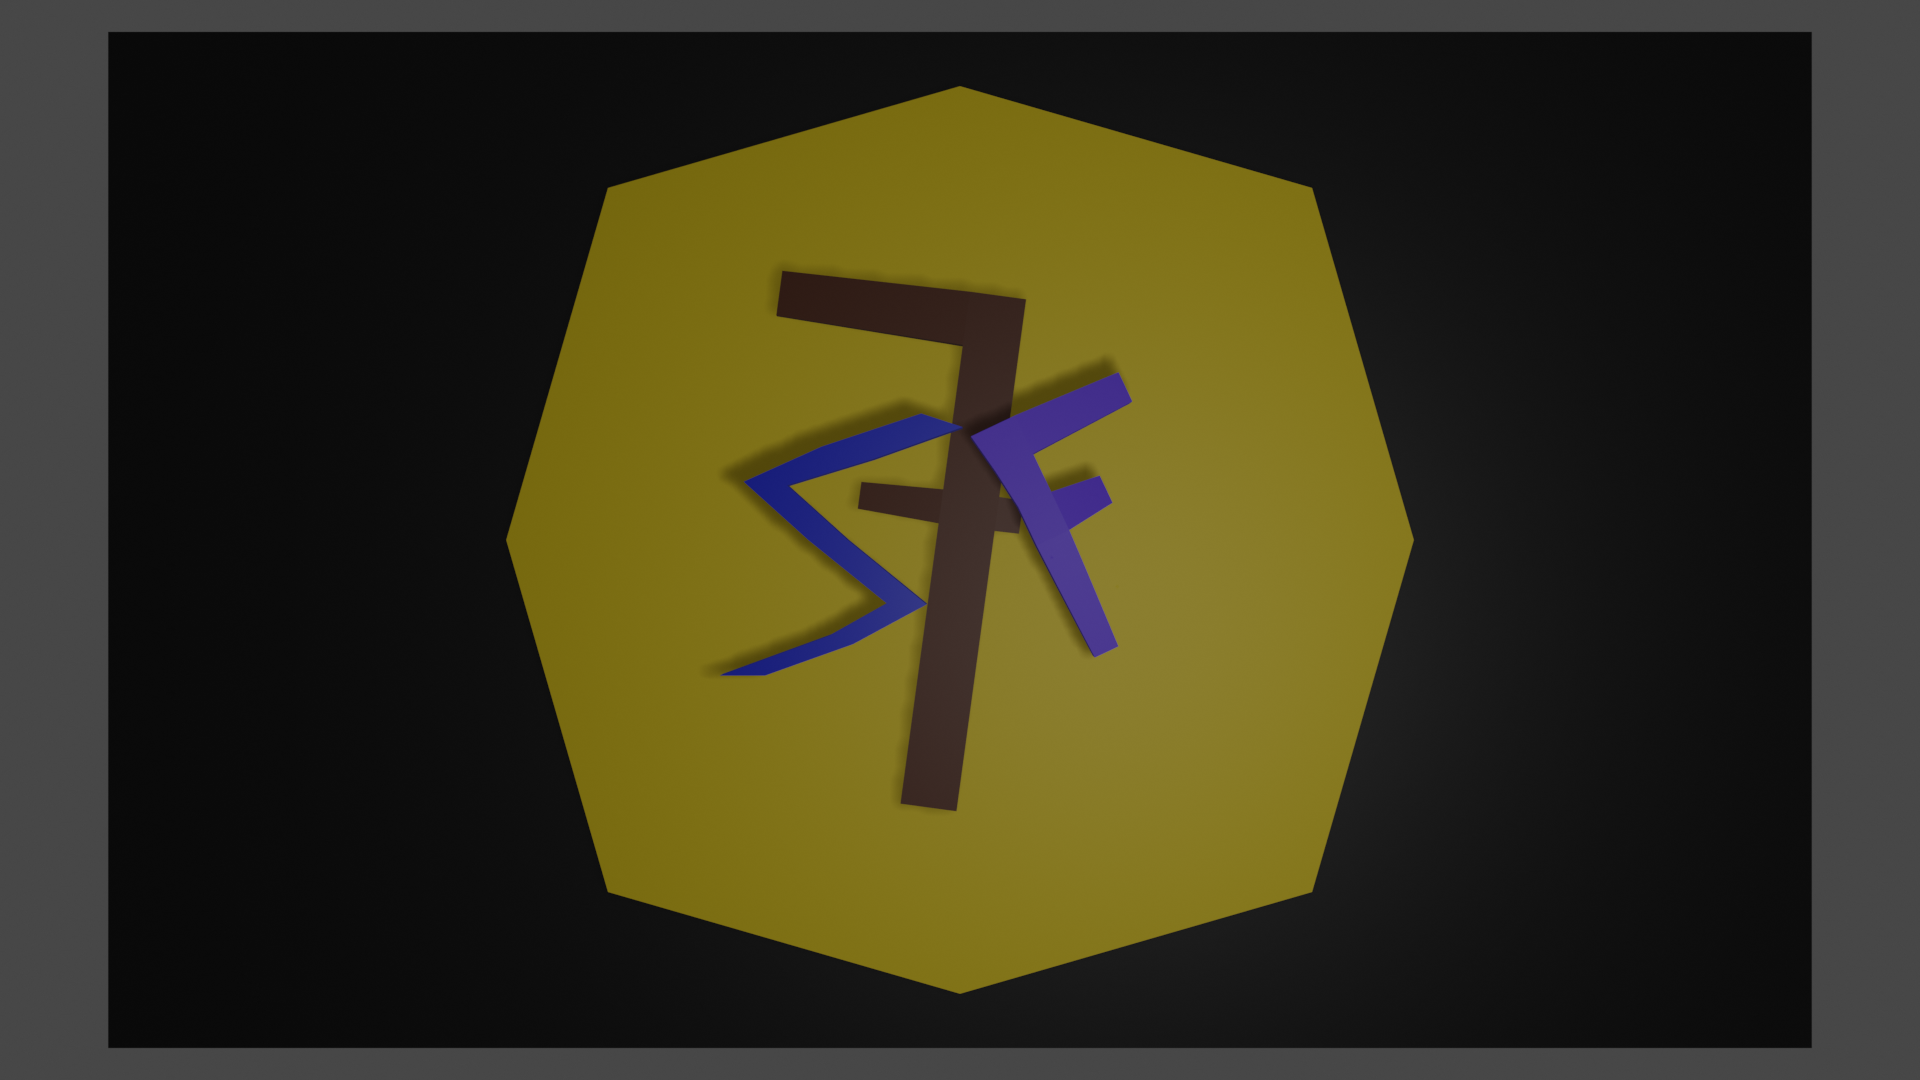
\includegraphics[width=8cm]{./images/logo.png}
    \vfill
    \vfill
\end{titlepage}

\section{Overview}

\subsection*{Theme, Setting, Genre}
We will be designing a 3d metroidvania platformer that takes place in a (mostly)
 renaissance medieval, high fantasy, setting. 

\subsection*{Core Gameplay Mechanics (Brief)}
The core gameplay will consist of going through dungeons to get a special item 
and killing the boss at the end of the dungeon. The dungeons will have at least 
two rooms with enemies and one puzzle room. The enemies you kill will drop 
health so as to keep the player playing aggressively rather than defensively. As
 you kill enemies you will get xp and you can use this to upgrade your skill 
 with your items. 

\subsection*{Target Platform \& Audience}
The game will be developed for PC using keyboard controls. Gamepad controllers 
will be implemented if time allows. \\

The game's target audience includes PC gamers who are fans of metroidvania
games like  \textit{Hollow Knight} and fans of adventure games with
combat/puzzle dungeons like the \textit{Legend of Zelda} series (particularly
entries like \textit{Ocarine of Time} and \textit{Twilight Princess}. We are
also designing our game to be played by an audience of college students and
professors with diverse gaming backgrounds (our classmates, our TAs, and our
instructor).

\subsection*{Project Scope}
The upper bound of the project's scope is:
\begin{itemize}
    \item Four unique bosses (two from a fantasy setting, two from a superhero setting)
    \item Four unique special items (two from a fantasy setting, two from a superhero setting)
    \item Four procedurally generated dungeons
\end{itemize}

The projects scope will begin much smaller and expand to the upper bound if time
and other resources allow. At a minimum, the projects scope will be:
\begin{itemize}
    \item Two unique bosses (one from a fantasy setting, one from a superhero setting)
    \item Two unique special items (one from a fantasy setting, one from a superhero setting)
    \item Two procedurally generated dungeons
\end{itemize}

Scope will expand first to three sets of bosses, unique items, and dungeons and
then expand to four if there is opportunity to expand the scope.

\subsection*{Game Time Scale}
There will be a working version of this game at the end of the 16 week time 
frame that is given.

\subsection*{Team Structure}
Jacob Santillanes (Ulteelectrom) is in the art section of the class and will be 
providing assets for the game. \\

Savanna Middaugh (savymidd) is in the art section of the class and will be 
providing assets for the game. \\

Hannah Murphy (murphy-97 on GitHub, HanJan on Discord) is in the programming
section of the class and will be implementing game systems in code and Unity.

\subsection*{Licenses/Hardware/Other Info}
The game will be made in Unity with assests created in Blender.  \\

Github repositiry: https://github.com/murphy-97/SuperFantasy7

\subsection*{Influences}
We took inspiration from several sources:

\begin{itemize}
    \item Metroidvania games: Our game will feature an open world of
    interconnected side-scolling platforming areas
    \item My Hero Academia, DC and Marvel: Half of the game premise draws from
    superhero media.
    \item Fantasy Genre: Half of the game premise draws from the fantasy genre.
    \item Skill Trees: Players will upgrade skills by spending points in a tree
    like in many other action-adventure games like Middle Earth: Shadow of
    Mordor and STAR WARS Jedi: Fallen Order.
    \item Legend of Zelda games: Dungeons feature puzzles, special items, and
    bosses.
    \item Rogue-like games: Dunegones are procedurally generated.
    \item Health Pickups: Players will recover health instantly from item
    pickups rather than maintaining an inventory, as in games like STAR WARS
    Battlefront (2004 and 2005 releases) and DOOM (2016). 
\end{itemize}

\subsection*{Elevator Pitch}

% In one or two paragraphs, describe the essence of your game idea. Try to capture
% what makes it interesting to your team and how the basic gameplay will work.
% State your “X” - both razor and slogan - as a part of your game description.
%
%   Razor:  "Superhero/medieval high fantasy metroidvania with puzzle/combat dungeons"
%   Slogan: "Realign the Worlds"

The game's working title is "Shattered Reformation." The slogan for the project
is "Relaign the Worlds." The razor to guide development is "Superhero/medieval
high fantasy metroidvania with puzzle/combat dungeons." \\

Dark lords shattered the Planar Focus, creating chaos in the multiverse and
causing two worlds to merge. You have to defeat them and collect the Shards of
Alignment to reassemble the Planar Focus. Only then will the worlds be returned
to their natural orders. \\

Players will gather the Shards of Alignment by defeating bosses at the end of
metroidvania-style dungeons. Players will learn new skills and abilities that
will evolve how they navigate the world and combat enemies. 

\section{Project Description}

\subsection{Rules \& Procedures}
Text goes here. Orion

\subsection{Sources of Conflict}
Text goes here. Jacob

\subsection{Unique Project Aspects}
% Premise: sci-fi plus fantasy
% Dungeons: balance between random generation and prefab set pieces
\begin{itemize}
	\item Features a mix of both classic fantasy and superhero themes.
	\item Uses randomised dungeons to deliver a unique experience in every game.
\end{itemize}

\section{Story \& Gameplay}
% Two worlds collided when the magic thingies were stolen
% The player must defeat fantasy monsters and super villains to bring alignment back to the multiverse
\subsection*{Story (Brief)}
The villains have merged two worlds together. One is a high fantasy setting and
one is a superhero setting. You need to separate the worlds and return
everything to normal. You play as either a hero or a knight. 

\subsection*{Gameplay (Brief)}
Basic platforming. The player can collect special items to interact with the
environment or find new ways of beating the enemies. The player will have a
basic attack, and a skill tree to upgrade their items and their basic attacks.  

\subsection*{Gameplay (Detailed)}
Text goes here. Savanna

\subsection*{Core Gameplay Loop}

\subsubsection*{Dungeon Gameplay Loop}
The majority of core gameplay occurs in the game's procedurally generated
dungeons. In these dungeons, players will encounter enemies, puzzles, special
items, and boss battles. The main challenge is derived from learning the
dungeon's layout to accomplish the player's goals within the dugeon. A typical
dugeon trek will have the following progression:

\begin{enumerate}
    \item Enter the dungeon
    \item Find and acquire the special item
    \item Find and defeat the boss
    \item Exit the dungeon and seek out the next dungeon in the overworld
\end{enumerate}

Navigating the dungeon to get from each of these steps to the next will require
the player to defeat enemies or solve puzzles in each room of the dungeon.

\subsubsection*{Overworld Gameplay Loop}
The gameplay loop that occurs between dungeons focuses on the player navigating
between dungeons. The player will explore the overworld to find the entrance of
each dungeon. Exploration in the overwold will focus on the player practicing
both combat and platforming mechanics as they move from platform to platform
defeating basic enemies between the last dugeon and the next.

\section{Schedule}
% Look at assignment due dates
% Start with two bosses and items
% Add a third boss and item if time
% Add a fourth boss and item if time

\subsection*{Phase 1: Conceptualization}

This phase is from 24 January 2020 through 10 February 2020. This phase will
flesh out early game design concepts, such as item, boss, and dungeons designs.
These assets will be designed mechanically and thematically, but no final coding
or art will be produced during this time.

\subsection*{Phase 2: Pre-Production}

This phase is from 10 February 2020 through 2 March 2020. This phase will
include development of early art assets and gray-box prototyping in Unity.
We will experiment with game systems and art individually.

\subsection*{Phase 3: Production}

This phase is from 2 March 2020 through 13 April 2020. This phase will see
finalization of assets, integration of assets in Unity, and full implementation
of all game mechanics. The game should be feature-complete by the end of this
phase.

\subsection*{Phase 4: Finalization}

This phase is from 13 April 2020 through 1 May 2020. No new features or assets
will be created during this time. Game features will be adjusted or fixed, and
that content which cannot be made playable will be cut.

% 03 Feb: Conceptualization 2
% 10 Feb: Conceptualization 3
% 24 Feb: Pre-Production 1
% 26 Feb: Midterm!
% 02 Mar: Pre-Production 2
% 23 Mar: Production 1
% 30 Mar: Production 2
% 06 Apr: Production 3
% 13 Apr: Production 4
% 27 Apr: QA/Polish 1
% 01 May: QA/Polish 2

\end{document}

    
